\chapter{Estudo dos Dados}
\label{cap:estudodados}


\section{Preparo dos Dados}


Os dados são anotados diariamente em planilhas para o controle da fábrica
de Cajati. Estes estão distribuídos em colunas com diversas propriedades analisadas em
laboratório de cada lote retirado da fábrica. Existem diversas planilhas para
lotes retirados de diversas partes do processo de fabricação. Devido a dificuldades logísticas de se casar um
mesmo lote de cimento em diferentes partes do processo (e.g. o mesmo lote ao
sair do forno e depois de finalizado e pronto para expedição), estudos serão feitos apenas para os dados de
\textit{expedição de cimento}. 

A Tabela~\ref{tb:vars} apresenta todas as variáveis, dependentes e independentes,
que serão usadas na modelagem.


\begin{table}[]
  \resizebox{\textwidth}{!}{\begin{tabular}{|l|llllll}
\cline{1-1}
\multicolumn{1}{|c|}{\textbf{ Variáveis (unidade)}}         &                                &                              &                           &                             &                               &                               \\ \hline
Composição Química (\%)                                   & \multicolumn{1}{l|}{$AL_20_3$} & \multicolumn{1}{l|}{$SIO_2$} & \multicolumn{1}{l|}{MGO}  & \multicolumn{1}{l|}{RICARB} & \multicolumn{1}{l|}{$P_2O_5$} & \multicolumn{1}{l|}{$F_2O_3$} \\ \hline
Água (\%)                                                 & \multicolumn{1}{l|}{AGP}       &                              &                           &                             &                               &                               \\ \cline{1-3}
Tempo até o começo e fim do endurecimento do material (s) & \multicolumn{1}{l|}{IP}        & \multicolumn{1}{l|}{FP}      &                           &                             &                               &                               \\ \cline{1-3}
Finura Blaine ($cm^{2}$/g)                                & \multicolumn{1}{l|}{SBL}       &                              &                           &                             &                               &                               \\ \cline{1-4}
Resistência Compressiva do Cimento (kPA)                  & \multicolumn{1}{l|}{RC3}       & \multicolumn{1}{l|}{RC7}     & \multicolumn{1}{l|}{RC28} &                             &                               &                               \\ \cline{1-4}
\end{tabular}}
\caption{Variáveis presentes nos dados de expedição de cimento cedidos pela Intercement}
\label{tb:vars}
\end{table}

Os dados de expedição de cimento são anotados aproximadamente por dia, possuindo 2520
entradas para 3650 dias distintos. Existem dias sem dados presentes. O
período contemplado pela planilha de dados vai do dia 02/01/2008 até o dia 29/12/2018.

\subsection{Dados faltantes}

Embora tenhamos uma quantidade razoável de dias com dados presentes, esses muitas vezes não possuem algum valor de alguma variável.
A seguir vemos para os dados de Expedição de Cimento, para cada uma de suas variáveis de entrada, a porcentagem de dados presentes. 


\begin{figure}[H]
  \centering
  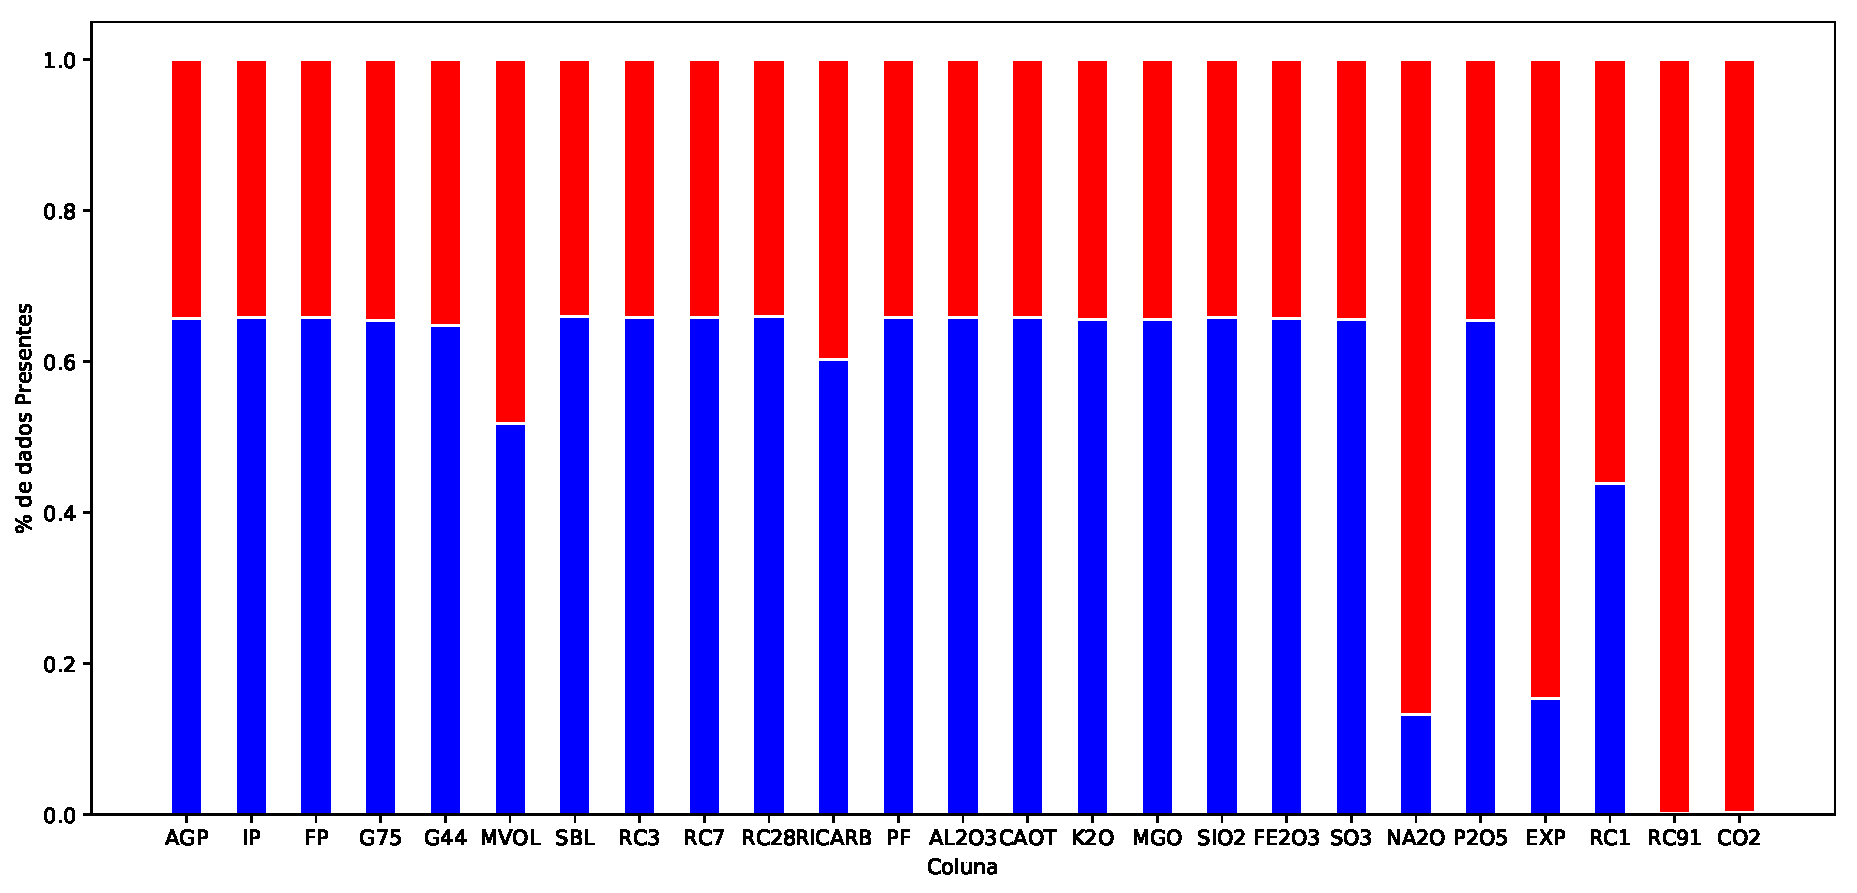
\includegraphics[width=0.9\columnwidth]{slides_dados_pct.pdf}
  \caption{Porcentagem de dados faltantes por variável para dados de Expedição
    de Cimento. Cada coluna azul indica a porcentagem do total de dias contemplados
    pela planilha que contém dados dessa variável.}
  \label{fig:dadosfalta}
\end{figure}


\section{Reamostragem dos dados}

Uma dos requisitos dos dados assumidos pelos modelos de séries temporais, que os mesmos
são espaçados regularmente pelo incremento de tempo escolhido, sem lacunas.
Portanto, os dados foram modificados para que entradas anotadas no mesmo dia
sejam unificadas em um único dia. Além disso, para dias no intervalo de tempo
estudado que não possuam entradas, foram criadas entradas com valores
artificiais que não perturbem a distribuição dos dados, e.g. os valores da
última entrada válida são copiados para frente até que se possua um novo valor.

A Figura \ref{fig:reamos} mostra como os dados estavam antes da reamostragem
para que eles se tornem diários: 

\begin{figure}[H]
  \centering
  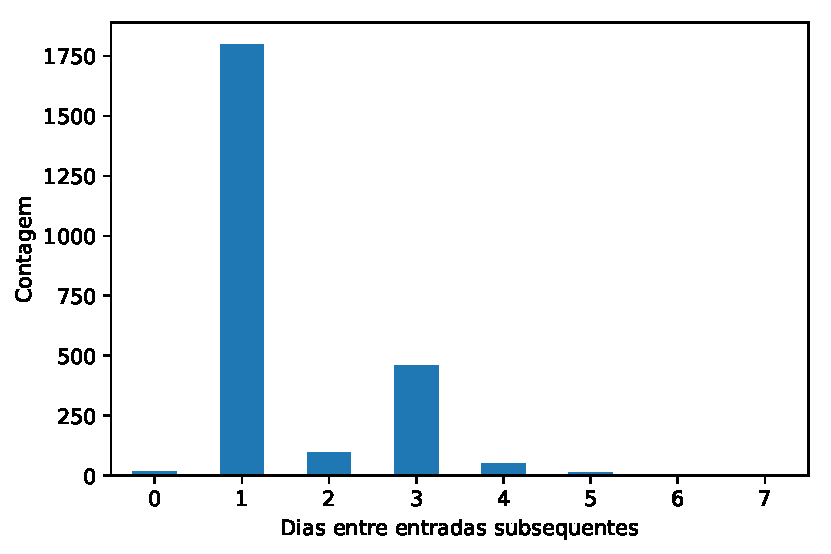
\includegraphics[width=0.5\columnwidth]{slides_dados_antes_resample.pdf}
  \caption{Distribuição das distâncias entre entradas subsequentes dos dados de
    Expedição de Cimento, antes da reamostragem. Grande parte das entradas da
    planilha estão distantes de 1 dia. Porém uma quantidade significativa tem 3
    dias de intervalo (sem dados no meio). Para o trabalho será necessário
    preencher esses dias faltantes.}
  \label{fig:reamos}
\end{figure}



\subsection{RC1, RC3, RC7 e RC28}

A variável de interesse para todos os modelos de predição é o RC28, o valor
escolhido por normas de segurança de construção civil. Os modelos usados nesse
trabalho irão buscar usar outros resultados de ensaios mais rápidos de
resistência compressiva na predição do ensaio mais importante e demorado. É
válido então uma análise de correlação entre essas grandezas.


A Figura~\ref{fig:gridcorr} mostra um correlograma entre os índices RC1, RC3 e RC7
atrasados e o RC28 diário. 

\begin{figure}[H]
  \centering
  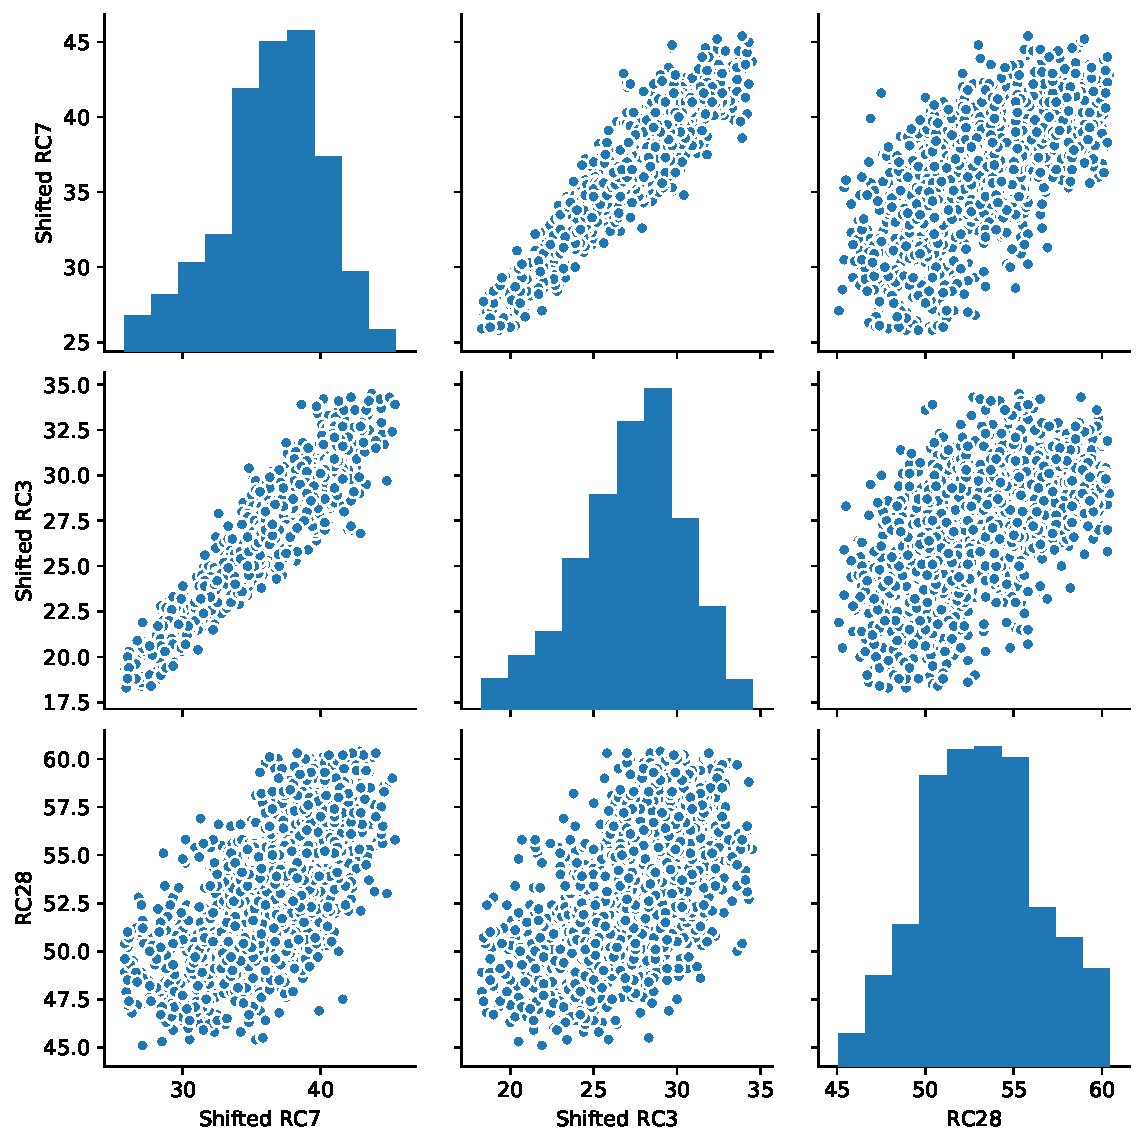
\includegraphics[width=0.9\columnwidth]{corr_grid.pdf}
  \caption{Correlograma dos índices de resistência compressiva. A diagonal
    mostra a distribuição de cada variável. Como esperado, RC28 tem uma
    correlação maior com ensaios mais recentes (i.e. RC7) do que com RC1.}
  \label{fig:gridcorr}
\end{figure}

A Tabela~\ref{tabelacorr} mostra o restante das correlações de Pearson \citep{dlbook} entre as demais
colunas de dados e o nosso objetivo, o índice RC28:


\begin{table}[H]
  \centering
\begin{tabular}{lr}
  \toprule
  {} &      RC28 \\
  \midrule
  AGP   &  0.592847 \\
  AL2O3 &  0.463414 \\
  P2O5  &  0.292252 \\
  SIO2  & -0.053178 \\
  MGO   & -0.371414 \\
  IP    & -0.132297 \\
  FP    & -0.419800 \\
  SBL   &  0.396555 \\
  PF    & -0.480720 \\
  \bottomrule
\end{tabular}
\caption{Tabela mostrando as correlações de Pearson entre cada uma das variáveis
  e o alvo RC28.} 
\label{tabelacorr}
\end{table}


É notável que o RC28 não possui uma alta correlação com nenhuma das propriedades
do cimento. Tendo essa correlação apenas com os outros índices de resistência compressiva.




%%% Local Variables:
%%% mode: latex
%%% TeX-master: "../quali"
%%% End:
